\documentclass{article}
\usepackage[utf8]{inputenc}

\usepackage{fullpage}
\usepackage{amsfonts, amsmath, pifont}
\usepackage{amsthm}
\usepackage{graphicx}
\usepackage{float}

\usepackage{tkz-euclide}
\usepackage{tikz}
\usepackage{pgfplots}
\pgfplotsset{compat=1.13}



\begin{filecontents}{q3.dat}
 n   xn 
 -1  0
 0   0
 1   -1  
 2   2
 3   0
 4   -4 
 5   0
 6   0
 7   3
 8   0
\end{filecontents}

\begin{filecontents}{q3_odd.dat}
 n   xn 
 -8  0
 -7   -1
 -6   0
 -5   0
 -4   2
 -3   0 
 -2   -1
 -1   0.5
 0   0
 1   -0.5  
 2   1
 3   0
 4   -2 
 5   0
 6   0
 7   1.5
 8   1110
\end{filecontents}




\begin{document}

\begin{figure}[h!]
    \centering
        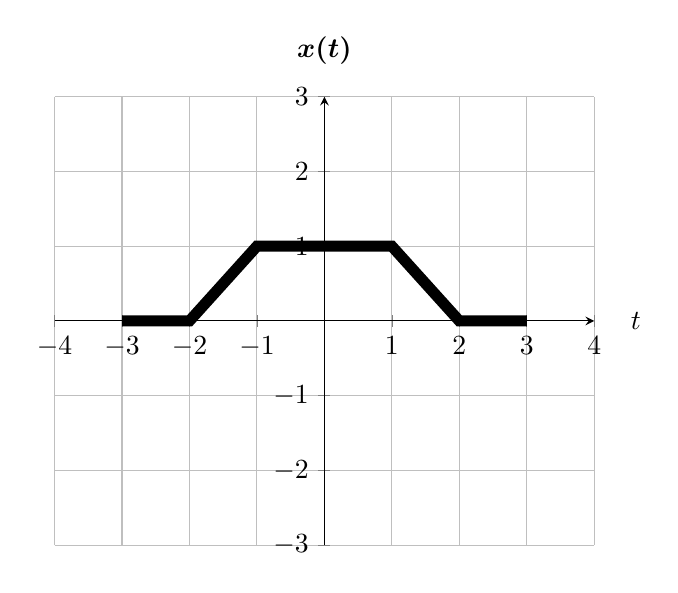
\begin{tikzpicture}[scale=1.0]
           \begin{axis}[
          axis lines=middle,
          xlabel={$t$},
          ylabel={$\boldsymbol{x(t)}$},
          xtick={-4, -3, -2, -1, ..., 4},
          ytick={-3, -2, -1, ..., 3},
          ymin=-3, ymax=3,
          xmin=-4, xmax=4,
          every axis x label/.style={at={(ticklabel* cs:1.05)}, anchor=west,},
          every axis y label/.style={at={(ticklabel* cs:1.05)}, anchor=south,},
          grid,
        ]
           \path[draw,line width=4pt] (-3,0) -- (-2,0) -- (-1,1) -- (1,1) -- (2,0) -- (3,0);
           \end{axis}
        \end{tikzpicture}
        \caption{$t$ vs. $x(t)$.}
        \label{fig:q2}
    \end{figure}

\begin{figure} [h!]
    \centering
    \begin{tikzpicture}[scale=1.0] 
      \begin{axis}[
          axis lines=middle,
          xlabel={$n$},
          ylabel={$\boldsymbol{x[n]}$},
          xtick={ -8, -7, ..., 8},
          ytick={-4, -3, -2, -1, ..., 4},
          ymin=-4, ymax=4,
          xmin=-8, xmax=8,
          every axis x label/.style={at={(ticklabel* cs:1.05)}, anchor=west,},
          every axis y label/.style={at={(ticklabel* cs:1.05)}, anchor=south,},
          grid,
        ]
        \addplot [ycomb, black, thick, mark=*] table [x={n}, y={xn}] {q3_odd.dat};
      \end{axis}
    \end{tikzpicture}
    \caption{$n$ vs. $Odd\{x[n]\}$.}
    \label{fig:q5}
\end{figure}



\begin{figure}[!htbp]
\begin{center}
\begin{tikzpicture}
    \begin{scope}[thick,font=\scriptsize]
    
    
    \draw [->] (-4,0) -- (4,0) node [above left]  {$\Re\{z\}$};
    \draw [->] (0,-4) -- (0,4) node [below right] {$\Im\{z\}$};

    
    \foreach \n in {-3,...,-1,1,2,...,3}{%
        \draw (\n,-3pt) -- (\n,3pt)   node [above] {$\n$};
        \draw (-3pt,\n) -- (3pt,\n)   node [right] {$\n i$};}
        
    \draw [thick, color=red] (0,0) -- (-1,1);
    \draw [color=blue, fill=blue] (-1,1) circle(0.05);
    \node [color=black] at (-1,1.3) {$ -1+i$};
\end{scope}
\end{tikzpicture}
\end{center}
\caption{ \textit{\textbf{$z=-1+i$}} is plotted on on the Complex Plane}
\end{figure}

\end{document}
